\chapter{Compilation Pipeline}
\label{chap:compilation_pipeline}

Here is the classical compiler pipeline :
\begin{figure}[H]
     \centering
     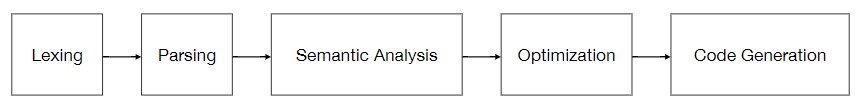
\includegraphics[scale=0.6]{pipeline.jpg}
     \caption{Compiler pipeline}
     \label{fig:compiler_pipeline}
\end{figure}
We will go through each step.

\section{Lexing}
    \theoremstyle{definition}
    \begin{definition}[Lexing]
        It's a lexical analysis, tokenization, scanning. It take the text and
        produce tokens (= "words"). e.g : foo = bar + 42 will produce |foo| = |bar| + |42|.
    \end{definition}
\section{Parsing}
    \theoremstyle{definition}
    \begin{definition}[Parsing]
        It take the output of lexing (tokens) and extract it's structure (by
        producing an Abstract Syntax Tree (AST)). It also catches syntax errors
        (like missing parenthesis around if in Java). Other kind of errors (like
        something that is not defined by the language) is not a syntax error,
        thus, the parser cannot cath it.
    \end{definition}
    \begin{figure}[H]
         \centering
         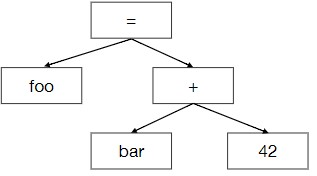
\includegraphics[scale=0.6]{parsing.jpg}
         \caption{Abstract Syntax Tree}
         \label{fig:ast}
    \end{figure}

    Note that lexing is optional while parsing (called scannerless parser) for
    others parsing is actually lexing AND parsing.
\section{Semantic Analysis}
    It consists of a series of check that is perform on the AST, two mains are
    Name binding et type checking.
    \subsection{Type checking}
    \theoremstyle{definition}
    \begin{definition}[Type checking]
        Verify that the type passed is what is expected.
        \begin{lstlisting}[language=Java]
            void print(String str)
            print(42)
        \end{lstlisting}
    \end{definition}
    \theoremstyle{definition}
    \begin{definition}[Type inference]
        Let the compiler guess the type of the variable given the context.
    \end{definition}
    Note that type checking is inference. When :
    \begin{lstlisting}[language=Java]
        String x = "foobar"
    \end{lstlisting}
    is used, it
    first need to guess what is "foobar", then check the consistency with the type.

    Sometimes, we need to know the return value's type of a function to perform
    the check. That's what Name Binding is.
    \subsection{Name Binding}
        \theoremstyle{definition}
        \begin{definition}[Name binding]
            Allow us to infer the type of a variable given the return type of a function.
        \end{definition}
        Note that it becomes much more complex with OOP.
    \subsection{Rest}
        It also performs flow check (missing return for example), access control
        (public, private, etc.).
\section{Optimization}
    Actually, the pipeline we saw in figure \ref{fig:compiler_pipeline} it's
    only the old school C compiler. New C compiler, do optimization on the
    produced machine code (LLVM, Low Level Virtual Machine)! Do not get confuse,
    it does not use a virtual machine at all... LLVM generate IR (intermediate
    representation), optimize it and then generate machine code.

    \begin{figure}[H]
         \centering
         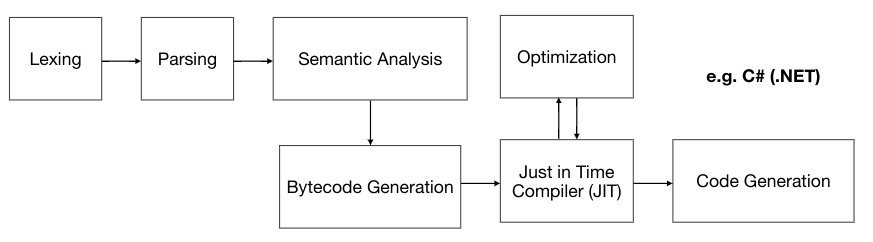
\includegraphics[scale=0.4]{csharp_pipeline.png}
         \caption{C\# pipeline}
         \label{fig:csharp_pipe}
    \end{figure}
    This one generate bytecode (Java name), that use useable but that
    won't be directly use by the machine. After the generation of the bytecode,
    it is passed to a Just In Time Compiler (JIT). What is done until JIT is
    done at compilation time, JIT and the following is done while running the program! 
    \begin{figure}[H]
         \centering
         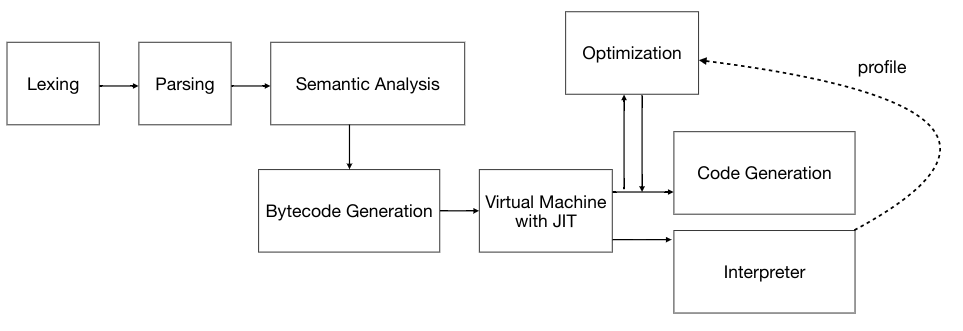
\includegraphics[scale=0.4]{java_python_pipeline.png}
         \caption{Java and Python pipeline}
         \label{fig:java_pipel}
    \end{figure}
    That's the architecture that most recent languages uses. The bytecode is
    passed to a VM executing a JIT. This VM can generate machine code (code
    generation) or pass it to in interpreter which will run a runtime profile
    that is much better for optimization! That the reason why Java can be as
    fast (or faster) the C. Pypy (Python), Java, TruffleRuby use this kind of
    architecture!

    We could also not optimize it! We could directly use the Tree-Walk
    interpreter, Ruby before 1.9 did that. CPython (standard one), and Ruby
    generate the bytecode and run it in a VM.

    \subsection{Tree-Walk Interpreter}
        Let's take the following program : 
        \begin{lstlisting}[language=Java]
            var foo = 42 + 52
            print(foo)
        \end{lstlisting}
        The AST is the following : 
        \begin{figure}[H]
             \centering
             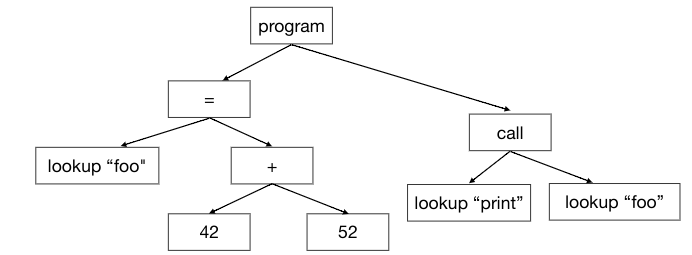
\includegraphics[scale=0.4]{ast_from_ex.png}
             \caption{Resulting AST}
             \label{fig:ast_from_ex}
        \end{figure}
        (Note that print has is own AST). We have the scope, containing the
        value of foo saved in the store and the definition of print. The
        procedure in order to execute is recursive, it will lookup for foo,
        perform the addition, store it. Lookup at the print definition, lookup
        for foo and foo will be passed as a parameter to print.
\section{Code Generation}
    It could be machine or bytecode generation.
    Example of Machine Code (e.g. x64) :
    \begin{lstlisting}[language=Java]
        int square(int num) {
            return num*num
        }
    \end{lstlisting}
    Becomes : 
    \begin{lstlisting}
        square(int):
            push    rbp
            mov     rbp, rsp
            mov     DWORD PTR [rpb-4], edi
            mov     eax, DWORD PTR [rpb-4]
            imul    eax, eax
            pop     rbp
            ret
        With optimization it becomes : 
            mov     eax, edi
            imul    eax, edi
            ret
    \end{lstlisting}

    While bytecode generation is:
    \begin{lstlisting}[language=Java]
        public class Hello {
            int square(int num) {
                return num*num
            }
        }
    \end{lstlisting}
    Which becomes (stacked base instead of registry based as before): 
    \begin{lstlisting}
        public class Hello {  
            public <init>()V
               L0    LINENUMBER 1 L0
                ALOAD 0    
                INVOKESPECIAL java/lang/Object.<init> ()V
                RETURN
               L1
                LOCALVARIABLE this LHello; L0 L1 0
                MAXSTACK = 1
                MAXLOCALS = 1
               square(I)I
                L0
                  LINENUMBER 3 L0
                  ILOAD 1
                  ILOAD 1
                  IMUL
                  IRETURN
                L1
                  LOCALVARIABLE this LHello; L0 L1 0
                  LOCALVARIABLE num I L0 L1 1
                  MAXSTACK = 2
                  MAXLOCALS = 2}
    \end{lstlisting}

    \section{Optimizations}
        As we have seen, we can optimize on tree or on target code. They are two
        types of optimization that are the base of everything : 
        \begin{itemize}
            \item Inlining : pulling a function in another one
            \item Partial evaluation : propagating known information (e.g constant-folding)
        \end{itemize}
        Some other exists like loop unrolling, etc.
        \subsection{Inlining}
            Take the following program : 
            \begin{lstlisting}
                var foo = false
                int a(){
                    if (foo) return somethingLongAndBoring()
                    else return b(true)+1
                }
                int b(boolean bar) {
                    return bar ? 42 : 52
                }
            \end{lstlisting}
            If we optimize the function a. It we online somethingLongAndBoring
            and b. However, if we do this and do not enter the condition, this
            could be bad for cache locality. Indeed, it will lead to a cache
            miss, with a lot of code, the time to retrieve the actual code will
            be huge. However, we know that foo is always false so we can get rid
            of the first condition! Then we can inline b. Thanks to the inlining
            of b, then constant folding it will lead on only this : 
            \begin{lstlisting}
                int a(){
                    return 43;
                }
            \end{lstlisting}
            Which is much more efficient! Thanks to that we can see that there
            is a complementarity between constant folding and inlining.